
%(BEGIN_QUESTION)
% Copyright 2006, Tony R. Kuphaldt, released under the Creative Commons Attribution License (v 1.0)
% This means you may do almost anything with this work of mine, so long as you give me proper credit

Voltage and current are related to one another {\it integral} function when dealing with capacitors and inductors.  Unlike resistors, where voltage and current simply follow one another in direct proportion, capacitors and inductors introduce the third variable of {\it time} into the relationships between voltage and current.

Determine which variable is the integral of which, for each of these circuits, by graphing both variables over time.  Then, write a calculus expression for each circuit showing the respective relationships between voltage and current.  Assume {\it perfect} capacitors and inductors, having no internal resistance or any other non-ideal characteristics:
 
$$\includegraphics[width=15.5cm]{i01569x01.eps}$$

$$\includegraphics[width=15.5cm]{i01569x02.eps}$$

Hint: remember these equations, which are akin to Ohm's Law for capacitors and inductors:

$$i = C {dv \over dt}$$

$$v = L {di \over dt}$$

\underbar{file i01569}
%(END_QUESTION)





%(BEGIN_ANSWER)

$$\includegraphics[width=15.5cm]{i01569x03.eps}$$

$$\includegraphics[width=15.5cm]{i01569x04.eps}$$

%(END_ANSWER)





%(BEGIN_NOTES)



%INDEX% Mathematics, calculus: derivative vs integral (applied to capacitors and inductors)

%(END_NOTES)


